\documentclass[uplatex, dvipdfmx]{jsarticle}

% --- 数学・統計 ---
\usepackage{amsmath, amssymb, amsthm}
\usepackage{bm}
\usepackage{mathtools}
\usepackage{enumitem}
\mathtoolsset{showonlyrefs=true}


% --- 図表 ---
\usepackage{tikz}
\usetikzlibrary{positioning, arrows.meta} 
\usepackage{graphicx}
\usepackage{float}
\usepackage{booktabs}
\usepackage[margin=25mm]{geometry}

% --- リンク ---
\usepackage{hyperref}
\usepackage{pxjahyper}

% --- tcolorbox (枠を作るパッケージ) ---
\usepackage{tcolorbox}
\tcbuselibrary{theorems, skins, breakable}

\tcbset{
  simple_style/.style={
    enhanced,
    breakable,
    frame hidden,
    colback=white,
    boxrule=0pt,
    boxsep=0pt,
    left=0pt,
    right=0pt,
    top=0pt,
    bottom=0pt,
    before skip=15pt,
    after skip=15pt,
    notitle,
  }
}

% --- カウンターを共通化する設定 ---

% 1. まずベースとなる「定義」を作る（これが親になります）
\newtcolorbox[auto counter, number within=section]{defn}[2][]{
  simple_style,
  before upper={\noindent\textbf{定義~\thetcbcounter：#2}\par\smallskip},
  #1
}

% 2. 「定理」は「定義」のカウンターを引き継ぐ
\newtcolorbox[use counter from=defn]{thm}[2][]{
  simple_style,
  before upper={\noindent\textbf{定理~\thetcbcounter：#2}\par\smallskip},
  #1
}

% 3. 「命題」も引き継ぐ
\newtcolorbox[use counter from=defn]{prop}[2][]{
  simple_style,
  before upper={\noindent\textbf{命題~\thetcbcounter：#2}\par\smallskip},
  #1
}

% 4. 「例」も引き継ぐ（左線あり）
\newtcolorbox[use counter from=defn]{exm}[2][]{
  simple_style,
  left=8pt,
  borderline west={0.5mm}{0pt}{black!30},
  before upper={\noindent\textbf{例~\thetcbcounter：#2}\par\smallskip},
  #1
}

\begin{document}

\section{なぜPearl流が必要か}
\subsection{因果とは何か}
「相関は因果を意味しない」これは多くの統計学の教科書に書かれている初等的な注意である.しかし，実際に単なる相関と因果の違いを説明するのは困難である.
これに対して，Rubinは次の平均処置効果(Average Treatment Effect: ATE)を因果効果として定義した.
\[
  ATE = E[Y^{(1)}-Y^{(0)}].
\]
ここで，$Y^{(1)}, Y^{(0)}$はポテンシャルアウトカムと呼ばれる変数である.
よく知られているように，Rubinの因果推論では，ポテンシャルアウトカムは同時に観測されず片方は必ず欠測するという欠測問題として因果推論の問題をとらえる.
この定義は式で書くと非常に明快であるが，因果と相関の違いは何かという根本的な問いに答えられていないようにも感じる.

\subsection{回帰係数は因果を意味するか}
我々が統計学や因果推論に期待することの一つは意思決定への寄与である.
つまり，原因となる変数が1単位変われば結果はいくら変わるのかという点である.
これは，直感的に単なる相関ではなく因果関係を要求することは想像に難くない.

何千回と擦られた例であるが，アイスクリームの消費量と溺死者数は因果関係でなく相関関係である.
つまり，行政の介入によりアイスクリームの流通を規制したとしても溺死者数を下げる結果には至らない.

\begin{figure}[htbp]
  \centering
  \includegraphics[width=0.8\columnwidth]{picture_1.png}
  \caption{アイスクリームの消費量と月別の溺死者数}
  \label{fig:picture_1}
\end{figure}

ところで，「原因となる変数が1変われば結果がいくら変わるのか」という文言は目的変数を説明変数で回帰したときの回帰係数の解釈として根付いている.
図\ref{fig:picture_1}を見れば，回帰係数は$0.04$であるから「アイスクリームの消費量を100円減らせば溺死者数が4人減る」という解釈ができる.

これは相関の意味では正しいといえるが，因果の意味では正しいとは言えない.換言すれば，観察の結果としての予測としては正しいが，原因に対する介入によって得られる結果の予測ではない.

線形回帰モデルの回帰係数に期待することが因果関係である場合，観察から得られた説明変数を全投入あるいはAICやBICによって変数選択することは得策とは言えない.

次のようなデータ生成を考えよう.
\begin{align}
  &\varepsilon_X, \varepsilon_Y, \varepsilon_1, \dots, \varepsilon_6 \overset{\text{i.i.d.}}{\sim} N(0, 1) \\
  X  &= 0.6Z_1 + 0.6Z_5 + \varepsilon_X \\
  Y  &= X + 0.6Z_2 + 0.6Z_3 + 0.6Z_6 + \varepsilon_Y \\
  Z_1 &= 0.6Z_2 + \varepsilon_1 \\
  Z_2 &= \varepsilon_2 \\
  Z_3 &= 0.5X + \varepsilon_3 \\
  Z_4 &= 0.7X + 0.7Y + \varepsilon_4 \\
  Z_5 &= \varepsilon_5 \\
  Z_6 &= \varepsilon_6 
\end{align}
ここで，変数そのものが$\varepsilon$として与えられた変数を\textbf{外生変数}という.
式では見にくいため，左辺を結果，右辺を原因として原因から結果へ矢線を引いて変数の関係を視覚的に表したグラフがG(図\ref{fig:dag_1})である.
\begin{figure}[htbp]
  \centering
  \begin{tikzpicture}[
    node_var/.style={circle, draw=none, minimum size=1cm, font=\large\bfseries},
    edge_path/.style={->, >=stealth, thick},
    node distance=2.0cm and 2.0cm
  ] 
    \node[node_var] (X) {$X$};
    \node[node_var, right=4.0cm of X] (Y) {$Y$};

    \node[node_var, above right=1.0cm of X] (Z1) {$Z_1$};
    \node[node_var, right=1.0cm of Z1] (Z2) {$Z_2$};

    \node[node_var, below right=of X, yshift=1.0cm] (Z3) {$Z_3$};
    \node[node_var, below right=of X] (Z4) {$Z_4$};

    \node[node_var, left=1.0cm of X] (Z5) {$Z_5$};
    \node[node_var, right=1.0cm of Y] (Z6) {$Z_6$};

    \node[node_var, above left=of X, yshift=-1.0cm] (G) {$G$};

    \draw[edge_path] (X) to (Y);
    \draw[edge_path] (Z2) to (Z1);
    \draw[edge_path] (Z1) to (X);
    \draw[edge_path] (Z2) to (Y); 

    \draw[edge_path] (X) to (Z3);
    \draw[edge_path] (Z3) to (Y);

    \draw[edge_path] (X) to (Z4); 
    \draw[edge_path] (Y) to (Z4);

    \draw[edge_path] (Z5) to (X);
    \draw[edge_path] (Z6) to (Y);
  \end{tikzpicture}
  \caption{データの生成過程}
  \label{fig:dag_1}
\end{figure}

図\ref{fig:dag_1}を見れば，どの矢線に沿って移動したとしても一周していないことが分かる.
これは，因果関係には原因と結果があり，一方向にしか進まないというある種哲学的な要請である.
このように頂点間の関係に向きがあり，どの矢線に沿って移動しても一周しないグラフを\textbf{非巡回有向グラフ}(Directed Acyclic Graph: DAG)といい，詳しい定義は3章で扱う.

$Y$と他の変数の関係は線形であるため，$Y$を説明変数とし，$X$と他の変数を説明変数とした重回帰分析を行えば$Y$と$X$の関係を捉えられるかもしれない.
今回はモデルの当てはまりの問題を考え，BICによる変数選択を行った.選ばれた変数とその偏回帰係数を表\ref{tab:results}に示す.

\begin{table}[htbp]
  \centering
  \caption{BIC最善モデルによるシミュレーション結果(n=10000)}
  \label{tab:results}
  \begin{tabular}{lccccc} % 6列分（左寄せ1つ + 中央揃え5つ）
    \hline
    項目 & $X$ & $Z_2$ & $Z_3$ & $Z_4$ & $Z_6$ \\ \hline
    偏回帰係数 & 0.3577 & 0.4029 & 0.3969 & 0.4619 & 0.4116 \\ \hline
  \end{tabular}
\end{table}

この偏回帰係数は因果的な関係ーXを1単位増加させればYは約0.358増加するーを表しているだろうか.
これを確かめるために，シミュレーションにより因果効果を導出してみよう.

次のようなデータの生成と対応するDAG $G_{\bar{X}}$ を考える.
\begin{align}
  &\varepsilon_Y, \varepsilon_1, \dots, \varepsilon_6 \overset{\text{i.i.d.}}{\sim} N(0, 1) \\
  X  &= x \\
  Y  &= X + 0.6Z_2 + 0.6Z_3 + 0.6Z_6 + \varepsilon_Y \\
  Z_1 &= 0.6Z_2 + \varepsilon_1 \\
  Z_2 &= \varepsilon_2 \\
  Z_3 &= 0.5X + \varepsilon_3 \\
  Z_4 &= 0.7X + 0.7Y + \varepsilon_4 \\
  Z_5 &= \varepsilon_5 \\
  Z_6 &= \varepsilon_6 
\end{align}

\begin{figure}[htbp]
  \centering
  \begin{tikzpicture}[
    node_var/.style={circle, draw=none, minimum size=1cm, font=\large\bfseries},
    edge_path/.style={->, >=stealth, thick},
    node distance=2.0cm and 2.0cm
  ] 
    \node[node_var] (X) {$X=x$};
    \node[node_var, right=4.0cm of X] (Y) {$Y$};

    \node[node_var, above right=1.0cm of X] (Z1) {$Z_1$};
    \node[node_var, right=1.0cm of Z1] (Z2) {$Z_2$};

    \node[node_var, below right=of X, yshift=1.0cm] (Z3) {$Z_3$};
    \node[node_var, below right=of X] (Z4) {$Z_4$};

    \node[node_var, left=1.0cm of X] (Z5) {$Z_5$};
    \node[node_var, right=1.0cm of Y] (Z6) {$Z_6$};

    \node[node_var, above left=of X, yshift=-1.0cm] (G) {$G_{\bar{X}}$};

    \draw[edge_path] (X) to (Y);
    \draw[edge_path] (Z2) to (Z1);
    \draw[edge_path] (Z2) to (Y); 

    \draw[edge_path] (X) to (Z3);
    \draw[edge_path] (Z3) to (Y);

    \draw[edge_path] (X) to (Z4); 
    \draw[edge_path] (Y) to (Z4);

    \draw[edge_path] (Z6) to (Y);
  \end{tikzpicture}
  \caption{介入後のデータの生成過程}
  \label{fig:dag_2}
\end{figure}

これは，$X$の値を強制的に$x$とした場合のデータの生成であり，構造方程式としては$X$のデータの生成過程を破棄して，$x$という値に固定したといえる.
このグラフ$G_{\bar{X}}$のデータの生成において，$x=1$のときの$Y$の平均値と$x=0$の場合の$Y$の平均値の差が実際の因果効果といえる.
精密な定義は第5章で与えられる.

実際に10000回のシミュレーションによって計算した結果は以下のとおりである.
\begin{figure}[htbp]
  \centering
  \includegraphics[width=0.8\columnwidth]{picture_2.png}
  \caption{ATEの計算結果}
  \label{fig:picture_2}
\end{figure}

図\ref{fig:dag_2}の計算結果により，真の因果効果ー$X$が1単位変化したときの$Y$の変化量ーは約$1.3$であることが分かる.
この値は先のBICによる変数選択によって得られた偏回帰係数$0.358$とは乖離しており，この偏回帰係数は因果的な解釈性を持たないことが分かる.

では，回帰係数に因果的な解釈ができる変数の組み合わせは存在するのであろうか.

\subsection{強く無視できる割り当て条件の謎}
次の\textbf{強く無視できる割り当て条件}はRubinの因果推論の中心的な仮定である.
\[
  (Y^{(1)}, Y^{(0)}) \perp X \mid Z.
\]
ただし，$X$は処置変数，$Z$は共変量である.この場合$Z$として選択してもよい変数はどんな変数であろうか.
図\ref{fig:dag_3},\ref{fig:dag_4}のデータ生成の場合でそれぞれ考えよう.

\begin{figure}[htbp]
  \centering
  \begin{minipage}[t]{0.48\textwidth}
    \centering
    \begin{tikzpicture}[
      node_var/.style={circle, draw=none, minimum size=0.8cm, font=\small\bfseries},
      edge_path/.style={->, >=stealth, thick},
      node distance=1.5cm and 1.5cm
    ] 
      \node[node_var] (X) {$X$};
      \node[node_var, right=4.0cm of X] (Y) {$Y$};
      \node[node_var, above right=0.5cm of X] (Z) {$Z$};
      \node[node_var, above left=0.8cm of Y] (Yp) {$(Y^{(1)}, Y^{(0)})$};
       
      \draw[edge_path] (X) to (Y);
      \draw[edge_path] (Yp) to (Y);
      \draw[edge_path] (Z) to (X);
      \draw[edge_path] (Z) to (Yp);
    \end{tikzpicture}
    \caption{交絡因子の構造}
    \label{fig:dag_3}
  \end{minipage}
  \begin{minipage}[t]{0.48\textwidth}
    \centering
    \begin{tikzpicture}[
      node_var/.style={circle, draw=none, minimum size=0.8cm, font=\small\bfseries},
      edge_path/.style={->, >=stealth, thick},
      node distance=1.5cm and 1.5cm
    ] 
      \node[node_var] (X) {$X$};
      \node[node_var, right=4.0cm of X] (Y) {$Y$};
      \node[node_var, above right=0.5cm of X] (Z) {$Z$};
      \node[node_var, above left=0.8cm of Y] (Yp) {$(Y^{(1)}, Y^{(0)})$};
       
      \draw[edge_path] (X) to (Y);
      \draw[edge_path] (Yp) to (Y);
      \draw[edge_path] (X) to (Z);
      \draw[edge_path] (Yp) to (Z);
    \end{tikzpicture}
    \caption{合流点の構造}
    \label{fig:dag_4}
  \end{minipage}
\end{figure}

図\ref{fig:dag_3}の場合は
\begin{align}
  &\varepsilon_X, \varepsilon_{Y_1}, \varepsilon_Z \overset{\text{i.i.d.}}{\sim} N(0, 1) \\
  Z &= \varepsilon_Z \\
  X &= \alpha_{XZ}Z + \varepsilon_X \\
  Y^{(1)} &= \alpha_{{Y_1}Z}Z + \varepsilon_{Y_1}
\end{align}
というデータの生成を考えれば，簡単な計算により条件付き独立性$Y^{(1)} \perp X \mid Z$が満たされていることが分かる.
ちなみに，第4,5章にて外生変数の正規性や構造方程式の線形性にとらわれずにより一般的な仮定の下で条件付き独立性が導かれる.

一方で，図\ref{fig:dag_4}の場合を考えみよう.次のデータの生成を考える.
\begin{align}
  &\varepsilon_X, \varepsilon_{Y_1}, \varepsilon_Z \overset{\text{i.i.d.}}{\sim} N(0, 1) \\
  X &= \varepsilon_X \\
  Y^{(1)} &= \varepsilon_{Y_1} \\
  Z &= \alpha_{ZX}X + \alpha_{Z{Y_1}}Y^{(1)} + \varepsilon_Z 
\end{align}
この場合は，$Y^{(1)} \perp X$が成り立っており，簡単な計算により条件付き独立性$Y^{(1)} \perp X \mid Z$が成り立たず，むしろ条件を付けることで独立性が崩れていることが分かる.

このように条件付き独立性はデータの生成過程と密接に関係していることが分かる.
では，DAGが与えられたときに条件付き独立性を保証するために必要な変数の集合はどんな集合であろうか.

\newpage

\subsection{Pearl流が解決するもの}
第1章を通して次のような疑問が浮かんでくる.
\begin{itemize}
  \item 因果効果とは何か？
  \item 回帰係数に因果的な解釈は求められるか？
  \item 強く無視できる割り当て条件を満足する変数の集合はどんな集合か？
\end{itemize}
Pearl流はこれらすべての疑問に(適切な仮定の下で)答えてくれる理論である.
本ゼミでは2章以降で以下の流れで章立てして進める(ことを目標にする).

第2章では，古典的な構造方程式モデリングを扱う.
第1章で見たようにDAGに基づいて，外生変数に正規分布を，変数間に線形性を仮定して解析を進める枠組みである.
構造方程式モデリングは，Pearl流因果推論における特殊な場合を扱っているに過ぎない.
しかし，グラフ構造と因果効果が綺麗に一対一対応する点，後の理論の基礎になっている点，歴史的経緯や第6章で扱うLiNGAMの理論において不可欠である点を鑑み取り上げることにした.
また，この章では第3章以降のグラフ理論の用語や定理が時々顔を覗かせるになるが，その点はご容赦願いたい.

第3章では，本ゼミで取り扱う範囲のグラフ理論の基礎を取り上げる.この章によってDAGの定義や性質が与えられる.

第4章では，ベイジアンネットワークを取り扱う.この理論の提唱者はJudeaPearl先生であり，グラフ構造に確率分布を対応させた理論である.
本章によって条件付き独立性とグラフ構造が対応することが分かる.

第5章では介入を取り扱う.
この章で与えられる介入及び因果効果の定義こそ「因果効果とはなにか？」という問いに対するPearl流における数学的な答えである.
また，この章で示されるバックドア基準によって選択される変数集合こそがその他の疑問に対する現代的な答えである.

第6章では因果探索について取り扱う.ここまでの議論はDAGが既知のものであるとしてきたが，因果探索は手元のデータからDAGの復元を試みる分野である.

\newpage

\section{構造方程式モデリング}

\begin{defn}{構造方程式}
  確率変数 $X_1, \dots, X_n$ と誤差項 $\varepsilon_1, \dots, \varepsilon_n$ について，次の関係が成り立つとする.
  \begin{align}
    \varepsilon_1, \dots, \varepsilon_n \overset{\text{i.i.d}}{\sim} \mathcal{N}(0, 1) \\
    X_i = \sum_{j < i} \beta_{ij} X_j + \varepsilon_i
  \end{align}
  この方程式を\textbf{構造方程式}という.また，係数 $\beta_{ij}$ をパス係数という.

また，$X = (X_1, \dots, X_n)^T, e = (\varepsilon_1, \dots, \varepsilon_n)^T$，$B = (b_{ij})_{i,j=1}^n$ を
\[
  b_{ij} = 
  \begin{cases} 
  \beta_{ij} & (j < i) \\
  0 & (\text{otherwise}) 
  \end{cases}
\]
とおいたときに，
\[
  X = BX + e
\]
と書ける.$B$ は\textbf{狭義下三角行列}である.
\end{defn}

$X_1, \dots, X_n$ について，構造方程式の右辺の変数から左辺の変数へ矢線を引きグラフを作ると，そのグラフは非巡回になる.
なぜなら，$X_i$ から $X_j$ への矢線が存在する場合 $i < j$ であるため，矢線に沿って移動したとき，添字は単調増加する.故に，巡回は発生しない.

逆に，DAGが与えられた場合でも，定理3.7に述べるトポロジカルソートを施すことにより，構造方程式の形で記述できる.
つまり，構造方程式においては，添字の大小は本質的ではなく，DAGとしての構造こそが本質的である.
また，下三角行列Bは重み付き隣接行列に対応する.

\begin{exm}{擬似相関}
  構造方程式が次のように定義されているとする：
  \begin{align}
    \varepsilon_1, \varepsilon_2, \varepsilon_3 \overset{\text{i.i.d.}}{\sim} \mathcal{N}(0, 1) \\
    \begin{cases}
    X_1 = \varepsilon_1 \\
    X_2 = \beta_{21} X_1 + \varepsilon_2 \\
    X_3 = \beta_{31} X_1 + \varepsilon_3
    \end{cases}
  \end{align}

  このとき，
  \begin{equation}
  E[X_2 X_3] = \beta_{21} \beta_{31}
  \end{equation}
  を $X_2, X_3$ の\textbf{擬似相関}という.

  この構造方程式に対応するDAGは以下の通りである.
  \begin{center}
  \begin{tikzpicture}[node distance=1.5cm, auto, >=latex, thick]
      \node (X1) {$X_1$};
      \node (X2) [below left=of X1] {$X_2$};
      \node (X3) [below right=of X1] {$X_3$};
      \draw[->] (X1) to (X2);
      \draw[->] (X1) to (X3);
  \end{tikzpicture}
  \end{center}
  この擬似相関は因果関係を意味しない.この相関は，$X_2$ と $X_3$ に共通の原因 $X_1$ が存在するために引き起こされる.
\end{exm}

\begin{exm}{直接効果・間接効果・総合効果}
  構造方程式が次のように定義されているとする：
  \begin{align}
    \varepsilon_1, \varepsilon_2, \varepsilon_3 \overset{\text{i.i.d.}}{\sim} \mathcal{N}(0, 1) \\
    \begin{cases}
    X_1 = \varepsilon_1 \\
    X_2 = \beta_{21} X_1 + \varepsilon_2 \\
    X_3 = \beta_{31} X_1 + \beta_{32} X_2 + \varepsilon_3
    \end{cases}
  \end{align}

  このとき，
  \begin{align}
    E[X_1 X_3] &= \beta_{31} E[X_1^2] + \beta_{32} E[X_1 X_2] + E[X_1 \varepsilon_3] \\
    &= \beta_{31} + \beta_{32} \beta_{21}
  \end{align}
  を $X_1$ から $X_3$ への\textbf{総合効果}という.

  対応するDAGは以下の通りである.
  \begin{center}
  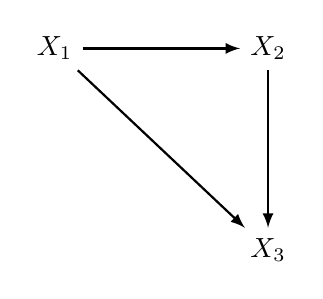
\begin{tikzpicture}[node distance=2cm, auto, >=latex, thick]
      \node (X1) {$X_1$};
      \node (X2) [right=of X1] {$X_2$};
      \node (X3) [below=of X2] {$X_3$};
      \draw[->] (X1) to (X2);
      \draw[->] (X2) to (X3);
      \draw[->] (X1) to (X3);
  \end{tikzpicture}
  \end{center}

  $X_3$ の構造方程式における $X_1$ の係数 $\beta_{31}$ を\textbf{直接効果}という.
  また，$X_1 \to X_2 \to X_3$ の有向道によって得られた $\beta_{32} \beta_{21}$ を\textbf{間接効果}という.

  より一般的に，構造方程式が以下で与えられるとする.
  \begin{align}
    \varepsilon_1, \varepsilon_2, \dots \varepsilon_n \overset{\text{i.i.d.}}{\sim} \mathcal{N}(0, 1) \\
    \begin{cases}
    X_1 = \varepsilon_1 \\
    X_2 = \beta_{21} X_1 + \varepsilon_2 \\
    \vdots \\
    X_m = \beta_{m, m-1} X_{m-1} + \varepsilon_m
    \end{cases}
  \end{align}
  このとき，
  \begin{equation}
    E[X_1 X_m] = \beta_{m, m-1} \cdot \beta_{m-1, m-2} \cdots \beta_{21}
  \end{equation}
  となり，これは $X_1$ から $X_m$ への間接効果である.
  総合効果こそ因果効果の大きさである.
\end{exm}

\begin{defn}{総合効果}
  構造方程式
  \begin{align}
    e &\sim \mathcal{N}(0, I_n) \\
    X &= BX + e
  \end{align}
  について，$n \times n$ 行列 $A$ を
  \begin{equation}
    A = (I - B)^{-1}
  \end{equation}
  とおいたときの $A$ の $(j, i)$ 成分 $a_{ji}$ を $X_i$ から $X_j$ への\textbf{総合効果}という.
\end{defn}

定義 2.4 の解釈は総合効果の本質を与える.
まず，$B$ は狭義下三角行列であるから冪零性により，
\begin{equation}
  (I - B)^{-1} = I + B + B^2 + \dots + B^{n-1}
\end{equation}
である.ここで$i<j$として$B^k$ の $(j, i)$ 成分 $b_{ji}^{(k)}$ に注目すると，
\begin{equation}
  b_{ji}^{(k)} = \sum_{l_{k-1}=1}^{n} \dots \sum_{l_1=1}^{n} \beta_{j, l_{k-1}} \beta_{l_{k-1}, l_{k-2}} \dots \beta_{l_1, i}
\end{equation}
となる.$B$ は狭義下三角行列であるため，
\begin{equation}
  b_{ji}^{(k)} = \sum_{i < l_1 < \dots < l_{k-1} < j} \beta_{j, l_{k-1}} \beta_{l_{k-1}, l_{k-2}} \dots \beta_{l_1, i}
\end{equation}
さて，各 $\beta_{j, l_{k-1}} \dots \beta_{l_1, i}$ が $0$ でない値を持つためには，任意の $\beta_{l_{m-1}, l_m}$ が $0$ でないことが条件となる.
これは，対応するDAGにおいて，
\begin{equation}
  X_i \to X_{l_1} \to \dots \to X_{l_{k-1}} \to X_j
\end{equation}
という長さ $k+1$ の有向道が存在することに等しい.
すなわち，$b_{ji}^{(k)}$ は $X_i$ から $X_j$ への長さ $k$ の有向道\footnote{第3章参照}によって得られる\textbf{間接効果}の和である.
したがって，
\begin{equation}
  (I - B)^{-1} = I + B + \dots + B^{n-1}
\end{equation}
の $(j, i)$ 成分は，長さ $1$ から $n$ の有向道によって得られる $X_i$ から $X_j$ への間接効果の和，つまり\textbf{総合効果}に等しい.

\begin{defn}{擬似相関}
  構造方程式
  \begin{align}
    e &\sim \mathcal{N}(0, I_n) \\
    X &= BX + e
  \end{align}
  において，$A = (I - B)^{-1}$ としたときに，
  \begin{equation}
    C = AA^\top - (A + A^\top) + I
  \end{equation}
  の $(j, i)$ 成分 $c_{ji}$ を $X_i$ と $X_j$ の\textbf{擬似相関}という.
\end{defn}

定義2.5\footnote{これは一般的な定義ではないことに注意されたい}を解釈しよう.まず，
\begin{equation}
  X = (I-B)^{-1}e = Ae
\end{equation}
より $X$ の分散共分散行列は，
\begin{align}
  E[XX^\top] &= E[(Ae)(Ae)^\top] \\
  &= A E[ee^\top] A^\top \\
  &= AA^\top
\end{align}
である.$i<j$として，$c_{ji}$ は $X_i$ と $X_j$ の共分散から，$X_i$ から $X_j$ への総合効果を引いたものである.
ここで，$A = (a_{ij})_{i,j=1}^n$ とおくと，
\begin{align}
  c_{ji} &= \sum_{k=1}^n a_{jk} a_{ik} - a_{ji} \\
  &= \sum_{k=1}^i a_{jk} a_{ik} - a_{ji} \\
  &= \sum_{k=1}^{i-1} a_{jk} a_{ik}
\end{align}
ここで，各 $k$ について，$a_{jk} a_{ik}$ は，$X_k$ から $X_i$ への総合効果と $X_k$ から $X_j$ への総合効果の積である.
これが $0$ でないときは，$X_k$ から $X_i$ への有向道が存在するかつ $X_k$ から $X_j$ への有向道が存在する場合である.
これは，$X_i$ と $X_j$ が共通の祖先を持つことを意味する\footnote{正確にはグラフ構造に対する忠実性の仮定が必要である}.

最後にパス係数の推定について少し触れよう.これまでは誤差項のパラメータは固定されていたが，推定論に関しては誤差項のパラメータも同時に推定する.
\begin{prop}{パス係数の推定}
  次の構造方程式を考える.
  \begin{equation}
      \varepsilon_1, \dots, \varepsilon_n \sim \mathcal{N}(\mu, \Psi)
  \end{equation}
  \begin{equation}
      \mu = (\mu_1, \dots, \mu_n), \quad \Psi = 
      \begin{pmatrix}
          \sigma_1^2 & & 0 \\
          & \sigma_2^2 & \\
          & & \ddots & \\
          0 & & & \sigma_n^2
      \end{pmatrix}
  \end{equation}
  \begin{equation}
      X = BX + e
  \end{equation}
  $B$ の非ゼロ成分を $\beta$ とおいて，$\theta = (\beta, \sigma_1^2, \dots, \sigma_n^2)$ とする.さらに，
  \begin{equation}
      \Sigma(\theta) = (I - B)^{-1} \Psi (I - B)^{-\top}
  \end{equation}
  とおいたときに，$\theta$ の最尤推定量 $\hat{\theta}$ は
  \begin{equation}
      f(\theta) = \text{tr}(\Sigma^{-1}(\theta) S) - \log(|\Sigma^{-1}(\theta) S|) - n
  \end{equation}
  を最小にする $\hat{\theta}$ として与えられる.ただし，$S$ は標本分散共分散行列である.
\end{prop}

\begin{proof}
  まず，
  \begin{equation}
      X = (I - B)^{-1} e
  \end{equation}
  より，$X \sim \mathcal{N}((I - B)^{-1} \mu, (I - B)^{-1} \Psi (I - B)^{-\top})$ である.
  ここで，標本 $x_1, \dots, x_p$ が与えられたとする.対数尤度関数は，
  \begin{align}
      -\log L(\theta) &= \frac{p}{2} \log (2\pi)^n |\Sigma(\theta)| + \frac{1}{2} \sum_{i=1}^p (x_i - \mu)^\top \Sigma^{-1}(\theta) (x_i - \mu) \\
      &= \frac{np}{2} \log 2\pi - \log |\Sigma(\theta)|^{-1} + \frac{p}{2} \text{tr} \left( \Sigma^{-1}(\theta) \cdot \frac{1}{p} \sum_{i=1}^p (x_i - \mu)(x_i - \mu)^\top \right) \\
      &= \frac{np}{2} \log 2\pi - \frac{p}{2} \log |\Sigma^{-1}(\theta)| + \frac{p}{2} \text{tr}(\Sigma^{-1}(\theta) S)
  \end{align}
  ゆえに，最尤推定量 $\hat{\theta}$ は，
  \begin{equation}
      -\log |\Sigma^{-1}(\theta)| + \text{tr}(\Sigma^{-1}(\theta) S)
  \end{equation}
  を最小化する $\theta$ として求められる.ここで，パラメータに関係ない項を加えて，
  \begin{align}
      f(\theta) &= \{ -\log |\Sigma^{-1}(\theta)| + \text{tr}(\Sigma^{-1}(\theta) S) \} - \log |S| - n \\
      &= \text{tr}(\Sigma^{-1}(\theta) S) - \log |\Sigma^{-1}(\theta) S| - n
  \end{align}
  を最小化する $\theta$ が最尤推定量である.
\end{proof}


1.2で考えた構造方程式において最尤法でパラメータを推定する.以下に構造方程式の再掲と，最尤法によるパス係数の推定の結果を記載する.
\begin{align}
    &\varepsilon_X, \varepsilon_Y, \varepsilon_1, \dots, \varepsilon_6 \overset{\text{i.i.d.}}{\sim} N(0, 1) \\
    X  &= 0.6Z_1 + 0.6Z_5 + \varepsilon_X \\
    Y  &= X + 0.6Z_2 + 0.6Z_3 + 0.6Z_6 + \varepsilon_Y \\
    Z_1 &= 0.6Z_2 + \varepsilon_1 \\
    Z_2 &= \varepsilon_2 \\
    Z_3 &= 0.5X + \varepsilon_3 \\
    Z_4 &= 0.7X + 0.7Y + \varepsilon_4 \\
    Z_5 &= \varepsilon_5 \\
    Z_6 &= \varepsilon_6 
  \end{align}

\begin{table}[htbp]
  \centering
  \caption{推定結果の要約}
  \label{tab:results_2}
  \begin{tabular}{lcccc}
    \hline
    結果 & 関係 & 原因 & 推定値 \\ \hline
    Z1 & $\leftarrow$ & Z2 & 0.589887 \\
    X & $\leftarrow$ & Z1 & 0.601150 \\
    X & $\leftarrow$ & Z5 & 0.596700 \\
    Z3 & $\leftarrow$ & X & 0.486784 \\
    Y & $\leftarrow$ & X & 1.007328 \\
    Y & $\leftarrow$ & Z2 & 0.581893 \\
    Y & $\leftarrow$ & Z3 & 0.597675 \\
    Y & $\leftarrow$ & Z6 & 0.600582 \\
    Z4 & $\leftarrow$ & X & 0.707937 \\
    Z4 & $\leftarrow$ & Y & 0.698095 \\ \hline
  \end{tabular}
\end{table}

\newpage

\section{DAG}

\begin{defn}{有向グラフ}
  \begin{enumerate}
      \item 有限集合 $V$ と $V \times V$ の部分集合 $E$ の組 $(V, E)$ を（有限）グラフ， $V$ の要素を\textbf{頂点}， $E$ の要素を\textbf{辺}という.
      \item $(X_i, X_j) \in E$ かつ $(X_j, X_i) \notin E$ であるとき， $X_i$ から $X_j$ へ矢線を引く.一方で， $(X_i, X_j), (X_j, X_i) \in E$ のとき， $X_i$ と $X_j$ の間に向きのない辺を引く.
      \item すべての辺が向きのある辺のとき， $G$ を\textbf{有向グラフ}という.
  \end{enumerate}
\end{defn}

\begin{figure}[htbp]
  \begin{minipage}{0.45\textwidth}
    \centering
      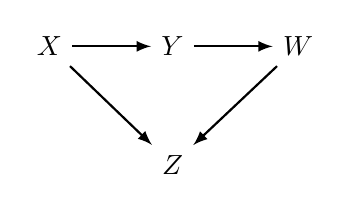
\begin{tikzpicture}[node distance=1cm, auto, >=latex, thick]
          \node (X) {$X$};
          \node (Y) [right=of X] {$Y$};
          \node (W) [right=of Y] {$W$};
          \node (Z) [below=of Y] {$Z$};
          \draw[->] (X) -- (Y);
          \draw[->] (Y) -- (W);
          \draw[->] (X) -- (Z);
          \draw[->] (W) -- (Z);
      \end{tikzpicture}
      \caption{有効グラフ}
  \end{minipage}
  \begin{minipage}{0.45\textwidth}
      \centering
      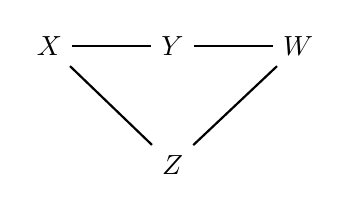
\begin{tikzpicture}[node distance=1cm, auto, thick]
          \node (X) {$X$};
          \node (Y) [right=of X] {$Y$};
          \node (W) [right=of Y] {$W$};
          \node (Z) [below=of Y] {$Z$};
          \draw[-] (X) -- (Y);
          \draw[-] (Y) -- (W);
          \draw[-] (X) -- (Z);
          \draw[-] (W) -- (Z);
      \end{tikzpicture}
      \caption{無向グラフ}
  \end{minipage}
\end{figure}

\begin{defn}{DAG}
$V = \{X_1, \dots, X_n\}$, $E \subset V \times V$, $G = (V, E)$ を有向グラフとする.
  \begin{enumerate}
      \item $X_i$ から $X_j$ への矢線が存在するとき， $X_i$ は $X_j$ の\textbf{親}であるといい， $X_j$ は $X_i$ の\textbf{子}であるという.また，
      \begin{equation}
          pa(X_j) = \{ X \in V \mid X \text{ は } X_j \text{ の親} \}
      \end{equation}
      と定義する.
      \item 頂点の列 $\{Y_i\}_{i=1}^m$ で，各 $i$ について， $Y_i$ から $Y_{i+1}$ または $Y_{i+1}$ から $Y_i$ への矢線が存在するとき， $\{Y_i\}_{i=1}^m$ を長さ $m$ の\textbf{道}という.とくに， $Y_i$ から $Y_{i+1}$ への矢線のみが存在する場合， $\{Y_i\}_{i=1}^m$ を\textbf{有向道}という.
      \item ある有向道 $\{Y_i\}_{i=1}^m$ が存在して， $Y_1 = Y_m$ となるとき，グラフ $G$ を\textbf{巡回グラフ}という.巡回グラフでない有向グラフを\textbf{非巡回有向グラフ}という.以下，非巡回有向グラフを \textbf{DAG} と表記する.
  \end{enumerate}
\end{defn}

\begin{figure}[H]
  \begin{minipage}{0.45\textwidth}
      \centering
      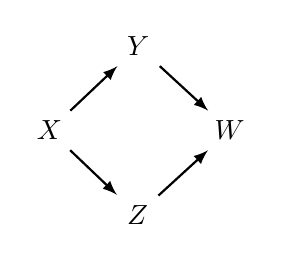
\begin{tikzpicture}[node distance=0.8cm, auto, >=latex, thick]
          \node (X) {$X$};
          \node (Y) [above right=of X] {$Y$};
          \node (Z) [below right=of X] {$Z$};
          \node (W) [below right=of Y] {$W$};
          \draw[->] (X) -- (Y);
          \draw[->] (Y) -- (W);
          \draw[->] (X) -- (Z);
          \draw[->] (Z) -- (W);
      \end{tikzpicture}
      \caption{巡回なし}
  \end{minipage}
  \begin{minipage}{0.45\textwidth}
      \centering
      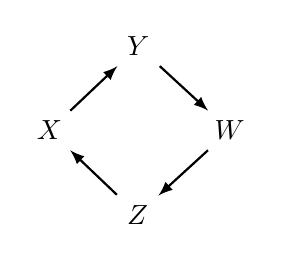
\begin{tikzpicture}[node distance=0.8cm, auto, >=latex, thick]
          \node (X) {$X$};
          \node (Y) [above right=of X] {$Y$};
          \node (Z) [below right=of X] {$Z$};
          \node (W) [below right=of Y] {$W$};
          \draw[->] (X) -- (Y);
          \draw[->] (Y) -- (W);
          \draw[->] (W) -- (Z);
          \draw[->] (Z) -- (X);
      \end{tikzpicture}
      \caption{巡回あり}
  \end{minipage}
\end{figure}

\newpage

\begin{defn}{子孫・先祖・合流点}
$V = \{X_1, \dots, X_n\}$, $E \subset V \times V$, $G = (V, E)$ は DAG であるとする.
  \begin{enumerate}
      \item 頂点 $X_i, X_j$ について，有向道 $\{Y_i\}_{i=1}^m, Y_1 = X_i, Y_m = X_j$ が存在するとき， $X_i$ は $X_j$ の\textbf{先祖}であるといい， $X_j$ は $X_i$ の\textbf{子孫}であるという.$X_i$ のすべての先祖を $an(X_i)$，すべての子孫を $de(X_i)$ で表す.
      \item すべての頂点から $X_i$ と $X_i$ の子孫を除いた頂点の部分集合を $nd(X_i)$ と書き， $nd(X_i)$ の要素を $X_i$ の\textbf{非子孫}という.
      \item 長さ $m$ の道 $\{Y_i\}_{i=1}^m$ について， $X_{j-1} \to X_j$ への矢線が存在し，かつ $X_{j+1} \to X_j$ への矢線が存在するとき， $X_j$ を\textbf{合流点（Collider）}という.とくに， $X_{j-1}$ と $X_{j+1}$ の間に辺が存在しないとき， $X_j$ を\textbf{V字合流点}という.
  \end{enumerate}
\end{defn}

\begin{exm}{子孫・非子孫・合流点}
  次の DAG を考える.
  \begin{center}
    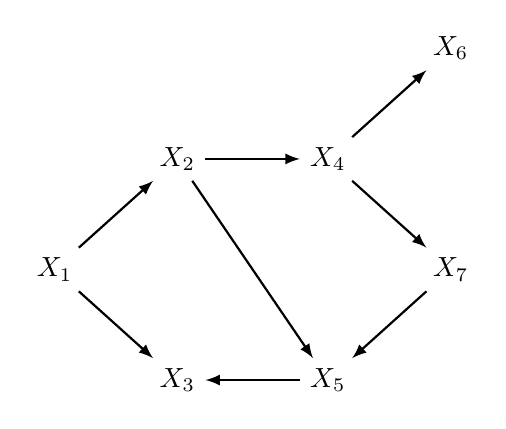
\begin{tikzpicture}[node distance=1.2cm, auto, >=latex, thick]
        \node (X1) {$X_1$};
        \node (X2) [above right=of X1] {$X_2$};
        \node (X3) [below right=of X1] {$X_3$};
        \node (X4) [right=of X2] {$X_4$};
        \node (X5) [right=of X3] {$X_5$};
        \node (X6) [above right=of X4] {$X_6$};
        \node (X7) [below right=of X4] {$X_7$};
        
        \draw[->] (X1) -- (X2);
        \draw[->] (X1) -- (X3);
        \draw[->] (X2) -- (X4);
        \draw[->] (X2) -- (X5);
        \draw[->] (X4) -- (X6);
        \draw[->] (X4) -- (X7);
        \draw[->] (X5) -- (X3);
        \draw[->] (X7) -- (X5);
    \end{tikzpicture}
  \end{center}

  \begin{enumerate}
      \item $X_1$ の子孫は？ $\Rightarrow \{X_2, X_3, X_4, X_5, X_6, X_7\}$
      \item $X_4$ の非子孫は？ $\Rightarrow \{X_1, X_2\}$
      \item 合流点は？ $\Rightarrow \{X_3, X_5\}$
  \end{enumerate}
\end{exm}

\begin{defn}{部分グラフ}
  $G = (V, E)$ をグラフとして，$V$ の部分集合 $U$ と
  \begin{equation}
    E_U = \{ (X_i, X_j) \in E \mid X_i, X_j \in U \}
  \end{equation}
  を定める.このとき，$G_U = (U, E_U)$ はグラフであり，$G_U$ を $U$ が生成する $G$ の\textbf{部分グラフ}であるという.
\end{defn}

\vspace{1em} 
$G$ が DAG であれば，部分グラフ $G'$ も DAG である.\\
（証明）
\begin{itemize}
    \item \textbf{有向グラフであること}：もし $(X_i, X_j) \in E', (X_j, X_i) \in E'$ であれば，$(X_i, X_j) \in E, (X_j, X_i) \in E$ となり，これは $G$ が有向グラフであることに矛盾する.
    \item \textbf{非巡回であること}：$G'$ が巡回グラフであるとすれば，有向道 $\{Y_i\}_{i=1}^m$ が存在する.ここで，各 $i$ について $Y_i \in V' \subset V$ かつ $(Y_i, Y_{i+1}) \in E' \subset E$ より，$\{Y_i\}_{i=1}^m$ は $G$ の有向道でもあるが，これは $G$ が非巡回であることに矛盾する.
\end{itemize}

\begin{defn}{隣接行列}
  $G = (V, E)$ をグラフ，$V = \{X_1, \dots, X_n\}$ とする.$n \times n$ 行列 $A$ を
  \begin{equation}
    a_{ij} = 
    \begin{cases} 
      1 & (X_j, X_i) \in E \\
      0 & (X_j, X_i) \notin E 
    \end{cases}
  \end{equation}
  として，$A = (a_{ij})_{i,j=1}^n$ で定義する.この $A$ をグラフ $G$ の\textbf{隣接行列}という.
\end{defn}

とくに，$G$ が DAG である場合，隣接行列は冪零行列である.これを証明するために，いくつかの補題を準備しよう.

\begin{prop}{トポロジカルソート}
  $G = (V, E)$ を DAG, $V = \{X_1, \dots, X_n\} \neq \emptyset$ とする.このとき，$X_1, \dots, X_n$ の順序を替えた $Y_1, \dots, Y_n$ であって，
  \begin{equation}
    (Y_i, Y_j) \in E \Rightarrow i < j
  \end{equation}
  となるようにできる.
\end{prop}

\begin{proof}
  まず，$pa(X_k) = \emptyset$ となる頂点 $X_k$ が存在することを証明する.\\
  任意の頂点 $X_i$ について $pa(X_i) \neq \emptyset$ と仮定する.
  $Z_1 \in V$ として，$pa(Z_1) \neq \emptyset$ より $(Z_2, Z_1) \in E$ となる $Z_2 \in V$ が存在.
  同様に $pa(Z_2) \neq \emptyset$ より $(Z_3, Z_2) \in E$ となる $Z_3 \in V$ が存在.
  これを繰り返すことで，有向道 $\{Z_i\}_{i=1}^{n+1}$ が存在する.一方で，$V$ の要素数は $n$ であったから，
  \begin{equation}
  Z_{i_1} = Z_{i_2}
  \end{equation}
  となる $i_1, i_2 \in \{1, \dots, n+1\}$ が存在する.これは $G$ が非巡回であることに矛盾する.

  さて，$V$ の要素数の帰納法によって補題を示す.このような規則でグラフの頂点の添字を付け替えることをトポロジカルソートという.
  \begin{itemize}
      \item $n=1$ のとき，$V$ は補題を満たす.
      \item $n=k$ のとき，$V$ は補題を満たすと仮定する.
      \item $n=k+1$ のとき，$G = (V, E)$ は DAG であるから，$pa(X_k) = \emptyset$ となる $X_k \in V$ が存在.
      このとき，$V' = V \setminus \{X_k\}$, $E' = \{ (X_i, X_j) \in E \mid X_i \neq X_k \text{ かつ } X_j \neq X_k \}$ とすれば，$G' = (V', E')$ は $G$ の部分グラフである.
      $G$ が DAG であったから $G'$ も DAG であって，要素数が $k$ である.
      ゆえに，$X_k = Y_1$ として，$V'$ をトポロジカルソート(命題3.7)して $\{Y_i\}_{i=2}^{k+1}$ と並べ替えれば，$\{Y_i\}_{i=1}^{k+1}$ はトポロジカルソートされた頂点集合となる.
  \end{itemize}
\end{proof}

\begin{thm}{}
  グラフ $G$ が DAG である場合，隣接行列 $A$ は\textbf{狭義下三角行列に相似}である.
\end{thm}

\begin{proof}
  $V = \{X_1, \dots, X_n\}$ とする.$\{Y_i\}_{i=1}^n$ はトポロジカルソートされたものであるとする.
  $Y_1, \dots, Y_n$ は $X_1, \dots, X_n$ の並べ替えであるから，$Y_1 = X_{\pi(1)}, \dots, Y_n = X_{\pi(n)}$ となるような$n$ 次対称群 $S_n$ の元 $\sigma$ が存在する.
  ここで，$P = (e_{\sigma(1)}, \dots, e_{\sigma(n)})$ とおく.
  つまり，$P = (p_{ij})_{i,j=1}^n$ とおくと，
  \begin{equation}
    p_{ij} = 
    \begin{cases} 
      1 & (j = \sigma(i)) \\
      0 & (\text{otherwise})
    \end{cases}
  \end{equation}

  ここで，$PAP^\top$ の $(i, j)$ 成分を $a'_{ij}$ とおく.
  \begin{align}
    a'_{ij} &= \sum_{k=1}^n \sum_{l=1}^n p_{ik} a_{kl} p_{jl} \\
    &= \sum_{k=1}^n p_{ik} \left( \sum_{l=1}^n a_{kl} p_{jl} \right) \\
    &= \sum_{k=1}^n p_{ik} a_{k, \sigma(j)} = a_{\sigma(i), \sigma(j)}
  \end{align}

  $a_{\sigma(i), \sigma(j)}$ の定義より，
  \begin{align}
    a_{\sigma(i), \sigma(j)} &= 
    \begin{cases} 
      1 & (X_{\sigma(j)}, X_{\sigma(i)}) \in E \\
      0 & (\text{otherwise})
    \end{cases} \\
    &= 
    \begin{cases} 
      1 & (Y_j, Y_i) \in E \\
      0 & (\text{otherwise})
    \end{cases}
  \end{align}

  ゆえに，$PAP^\top$ は $\{Y_i\}_{i=1}^n$ のグラフの隣接行列 $A'$ に等しい.
  ここで，$\{Y_i\}_{i=1}^n$ はトポロジカルソートされているため，
  \begin{equation}
    (Y_j, Y_i) \in E \Rightarrow j < i
  \end{equation}
  ゆえに，$A'$ は狭義下三角行列である.したがって，隣接行列$A$は狭義下三角行列に相似である.
\end{proof}

\end{document}